\documentclass[sigconf,nonacm]{acmart}

\usepackage{booktabs} % For formal tables
\settopmatter{printacmref=false}
% TOG prefers author-name bib system with square brackets
\citestyle{acmauthoryear}
%\setcitestyle{nosort,square} % nosort to allow for manual chronological ordering



\usepackage[ruled]{algorithm2e} % For algorithms
\renewcommand{\algorithmcfname}{ALGORITHM}
\SetAlFnt{\small}
\SetAlCapFnt{\small}
\SetAlCapNameFnt{\small}
\SetAlCapHSkip{0pt}


% Copyright
%\setcopyright{acmcopyright}
%\setcopyright{acmlicensed}
%\setcopyright{rightsretained}
%\setcopyright{usgov}
%\setcopyright{usgovmixed}
%\setcopyright{cagov}
%\setcopyright{cagovmixed}

% DOI
%\acmDOI{0000001.0000001_2}

% Paper history
%\received{February 2007}
%\received{March 2009}
%\received[final version]{June 2009}
%\received[accepted]{July 2009}


% Document starts
\begin{document}
	% Title portion
	\title{Sparse Voxel Octree GPU Ray Marching}
	
	% DO NOT ENTER AUTHOR INFORMATION FOR ANONYMOUS TECHNICAL PAPER SUBMISSIONS TO SIGGRAPH 2019!
	\author{Thomas Conrad}
	\affiliation{%
		\institution{Oregon State University}
		\city{Corvallis, OR}
		\postcode{2800}
		\country{USA}}
	\email{conradth@oregonstate.edu}
	
	
	\begin{teaserfigure}
		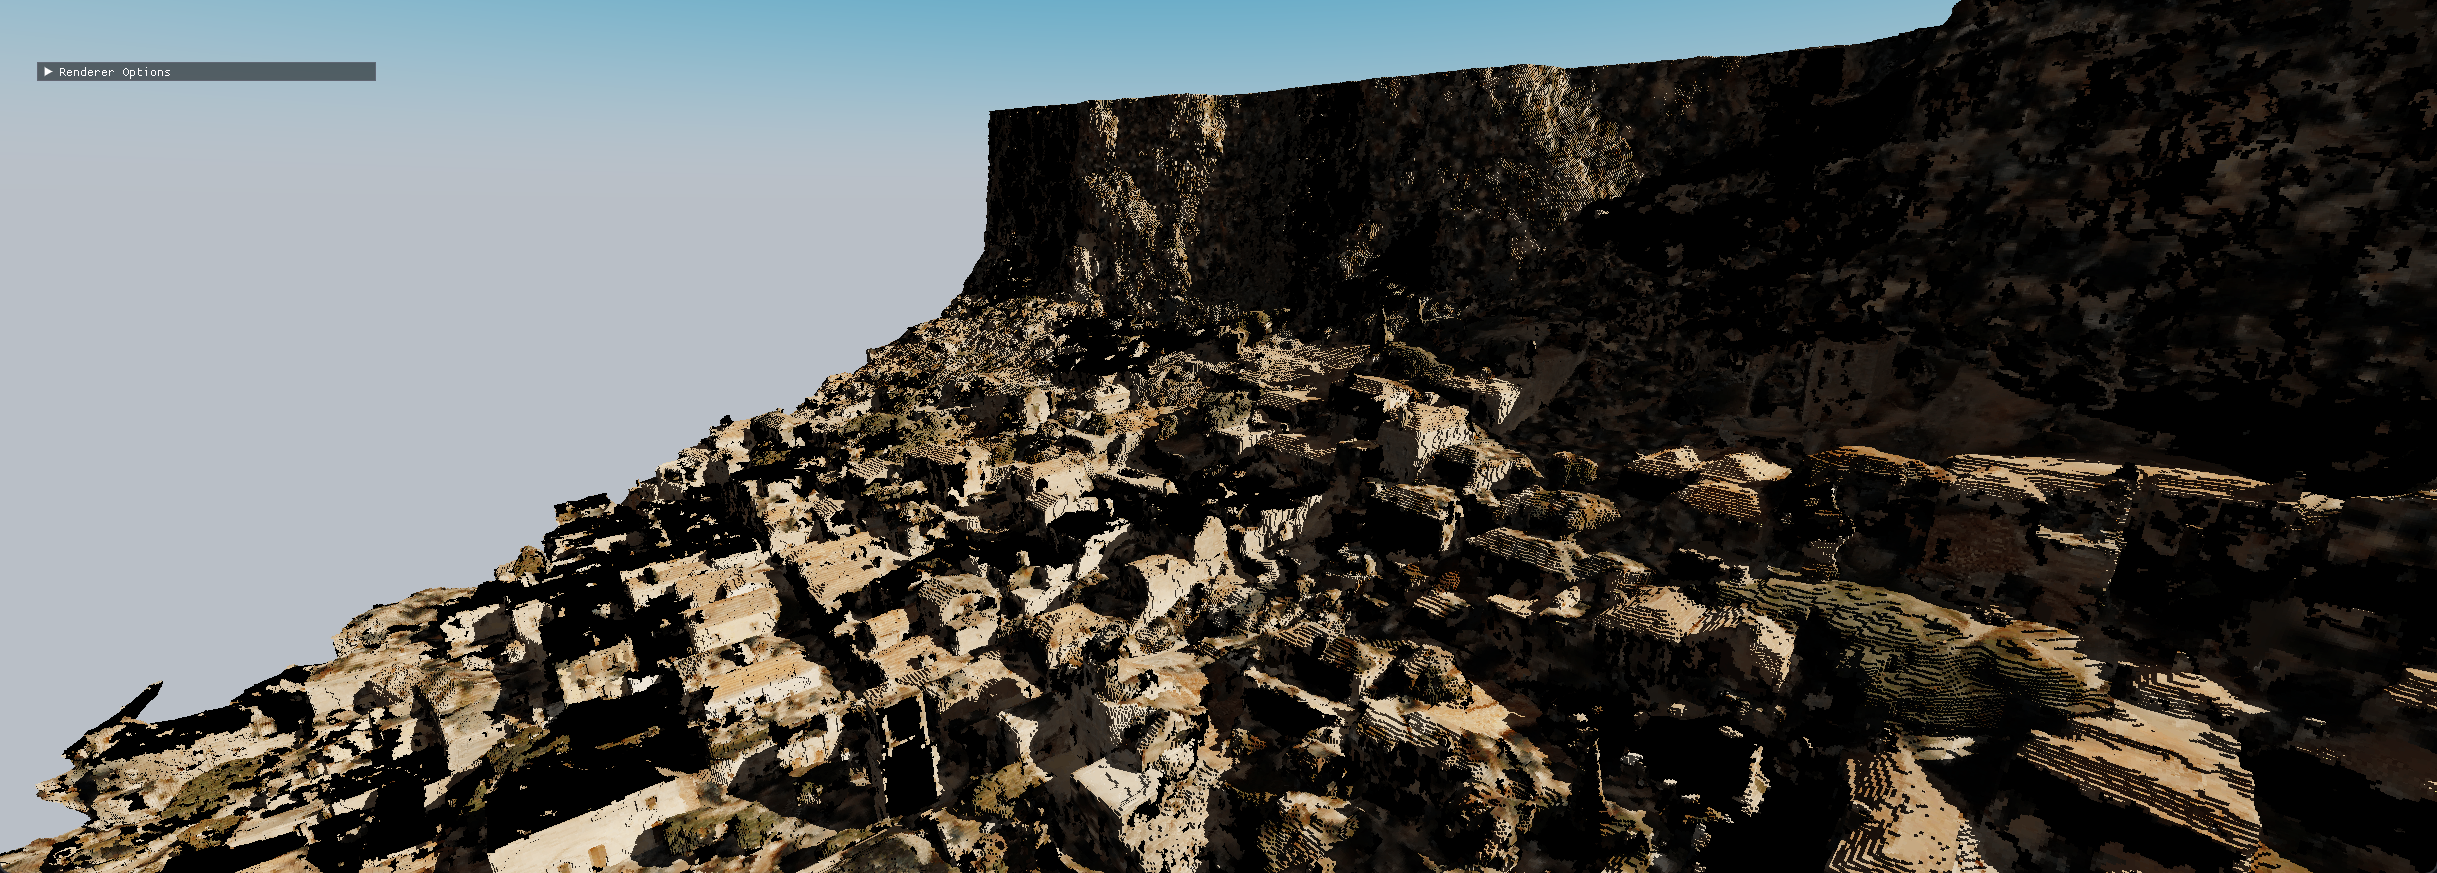
\includegraphics[width=\textwidth]{town}
		\caption{A large town scene \cite{monemvasia_town_scene_nodate} converted to a .vox file and loaded into my renderer. The black areas are caused by errors in the conversion process from a mesh to a voxel tree.}
		\label{fig:town}
	\end{teaserfigure}
	
	\begin{abstract}
		This project seeks to investigate the viability of implementing a sparse voxel cone tracing technique in a gpu fragment shader for global illumination approximation. The aim is to assess the performance and features of the technique, and to determine if it is suitable for practical use in modern gaming. To accomplish this, a sparse voxel cone tracing based GI renderer will be implemented within the given timeframe and the results will be evaluated. The project will also provide insight into the limitations of the technique and how it can be improved in the future. In the end voxel cone tracing wasn't implemented as the time limit was hit, but raytracing with shadows was implemented in a shader, which showed around a 20-times performance improvement compared to the same code running on the CPU.
	\end{abstract}
	
	\begin{CCSXML}
		<ccs2012>
		<concept>
		<concept_id>10010147.10010371.10010372.10010374</concept_id>
		<concept_desc>Computing methodologies~Ray tracing</concept_desc>
		<concept_significance>500</concept_significance>
		</concept>
		</ccs2012>
	\end{CCSXML}
	
	\ccsdesc[500]{Computing methodologies~Ray tracing}
	
	%
	% End generated code
	%
	
	
	\keywords{Sparse Voxel Octree, Ray Tracing}

	\maketitle
	
	
	
	
\section{Motivation}
Currently in gaming, ray traced shadows and reflections is the main area of innovation. In \cite{10.1145/2037826.2037853}, a novel method for approximating path traced global illumination was proposed. However, the use of this technique was ultimately abandoned due to the limited GPU power at the time, as well as the method's various technical drawbacks such as high memory usage, susceptibility to memory leaks, costly anisotropy, difficulty of use, expensive dynamic objects, and lack of control. Attempts to implement voxel-based rendering in game engines initially began with Unreal Engine 4; however, this was eventually abandoned due to practical limitations. Unity also experimented with a voxel-based rendering system called SEGI, while CryEngine implemented a variant. Ultimately, voxel-based rendering was unsuccessful due to its limited practical applications. The recent implementation of RTX technology has led to a decrease in research devoted to alternative GI solutions. Although it is widely believed that raytracing is the future of rendering, further hardware development and research is needed before it can be used in real-time applications. 

The sparse voxel cone tracing technique for GI approximation, introduced over 10 years ago, has since been implemented in the Godot engine. As GPU performance is now much higher than in 2011, when the GTX 580 was released, sparse voxel cone tracing may now be viable for implementation in the average machine. This project aims to implement as much of a sparse voxel based GI renderer as possible within a given timeframe and assess the results.
\section{Previous works}
\subsection{Gigavoxels}
In 2009 the Gigavoxels paper was one of the first publications that dealt with sparse voxel octrees.

The main ideas presented in the paper are: 
\begin{enumerate}
	\item A hierarchical data structure called GigaVoxels is used to store voxel-based data. This structure allows for efficient representation of the data and allows for fast streaming of the data.
	\item Ray-guided streaming of the data is used to efficiently render the data. This allows for efficient rendering of detailed voxel-based data.
	\item A GPU-based implementation of the GigaVoxels system is presented. This allows for improved performance and real-time rendering of the voxel-based data.
	\item A set of optimizations are presented to improve the performance of the GigaVoxels system. These optimizations include support for partial update of the voxel data and multi-resolution rendering techniques.
\end{enumerate}

\subsection{Sparse Voxel Octrees}
The Indirection Pool \cite{10.5555/1062395} is a memory pool that is used to store pointers to dynamically allocated data structures, such as linked lists and trees. The pool works by allocating a single block of memory for all the pointers and then mapping each pointer in the pool to an index. This allows for efficient lookups of pointer data structures by their index. It was presented by Cyril Crassin the same person who was the main author behind both the cone tracing and gigavoxel papers. The guy really liked voxels, apparently. The indirection pool implementation is heavily optimized by using a suite of tricks, like using a 3d texture sampler for the pool as all values are 32 bits, the same as an rgba value, and utilizing UV-tiling to only use the fractional part of the lookup coordinate. I considered using the indirection pool to hold my SVO, but decided against it as it seemed more cumbersome that it needed to be and like it would be hard to expand my implementation later. Perhaps in a time before SSBO's it might have been the only way to sample buffers larger than the uniform buffer size limit.
\subsection{NVidia Voxel Cone Tracing}

The Nvidia voxel cone tracing article \cite{10.1145/2037826.2037853} discusses a new method for interactive indirect illumination. It is a technique that combines the advantages of voxel cone tracing and a sparse voxel representation to achieve real-time indirect illumination. It allows for efficient sampling, accurate lighting, and fast rendering. The results show that the method can be used to create realistic indirect illumination in real-time, and has the potential to be used in a variety of applications. The paper seemed quite ahead of its time, as it achieved actual real time global illumination at a point where Pixar was just beginning to use ray traced lighting. 

\section{Methods}
\subsection*{Graphics Engine}
The voxel renderer utilizes the Vulkan API as a graphics backend. \url{vulkan-tutorial.org} \cite{VKTUT} was consulted to learn about the Vulkan API and how to implement it, yet getting a static triangle to be displayed on screen took considerable time due to the extreme verbosity of Vulkan. The experience gained from using Vulkan in this project has allowed my to build most applications in Vulkan, however, the OpenGL API is simpler and quicker for prototyping, and so is likely to remain my preferred choice for prototyping applications. This should minimize any potential failure points as Vulkan and the algorithm will not have to be addressed simultaneously. \\
\\
Initially I wanted to go with Vulkan for its universal Ray Tracing extensions which might be useful in speeding up intersection tests. After looking into the subject I realized that it was an extremely difficult thing to get working with a non-standard acceleration structure, like that sparse voxel octree that I had implemented, and I therefore scrapped the idea of using hardware raytracing, and went for a heavily optimized software based solution running in the fragment shader. 

\subsection*{Sparse Voxel Octree Implementation}
A sparse voxel octree is a tree-like data structure that is used to store a three-dimensional grid of voxels. Voxels are small, volumetric units that are used to represent 3D objects.

The octree is composed of nodes, which are structs that contain pointers to their parent node and to their children or data, depending on whether the node is a leaf or not. When inserting a voxel in the octree, the tree can be recursively traversed to find the octant that contains the voxel coordinate. As the tree is traversed, new nodes are allocated as needed. When the predefined maximum depth of the tree is reached, space is allocated for the voxel data at that location.

Retrieving data from the octree works in a similar way, but instead of allocating new nodes, the traversal is simply stopped if an empty octant is encountered. This allows for efficient storage and access of the voxel data in the grid.

The use of a sparse voxel octree can provide a memory and performance tradeoff when compared to other methods of storing and manipulating voxel data. Because the octree only allocates nodes and data for occupied voxels, it can be more memory-efficient than storing the entire voxel grid in memory, even if the grid is mostly empty. This can be particularly useful for large voxel grids or for applications where memory usage is a concern.

However, there are also performance tradeoffs to consider when using a sparse voxel octree. Traversing the tree to insert or retrieve data can take longer than accessing a flat array of voxel data, particularly for large octrees with many levels. This is because the index in a dense array can be directly calculated from a location in $O(1)$ time, whereas the sparse array will have to do a full tree traversal, performing $O(\log n)$ checks, where n is the voxel side length. Additionally, the use of pointers to link nodes and data can also introduce some overhead, particularly in languages that do not have native support for pointer arithmetic, which I experienced when porting my implementation to the GPU.

For Ray Traversal a sparse voxel octree makes a lot of sense due to the efficient traversal algorithm, which is why it was chosen. The memory efficiency is a very nice bonus.

The CPU based implementation that I implemented is a pointer based structure. Each node either holds eight voxels or eight pointers to child nodes, depending on whether it's a leaf or not. This means that each leaf has eight voxels, which will sometime speed up lookup results because of cpu caching. In ray traversal neighboring nodes are often accessed in sequence. This is an advantage to dense octrees, but for SVO's, including pointers to the neighboring nodes can speed up the lookup time.

\subsection*{Contiguous Sparse Voxel Octree}
To copy the octree to the GPU the memory needs to be located along a contiguous array in memory. The way to do this is to create some struct that can hold the data in an octree node and save it in an array. That array can then be sent to a storage buffer on the GPU to load the data. It is here very important to use the std\_430 specification for the storage buffer, as otherwise the memory alignement is not guaranteed to fit. In general it is important to check that the memory alignment is the same for the struct on the cpu and gpu. Inspired by Nvidias indirection pool \cite{10.5555/1062395}, I implement each node as grid consisting of nine cells, one for mipmapping and 8 for the octants. Each cell is a 32bit unsigned integer. The last byte represents the type of the cell. The cell type can either be an empty leaf, a solid leaf (voxel), or branch containing a pointer to a child grid. In the case where the cell directs to a voxel the first three bytes represent an 8-bit rgb color. In the case where the the cell directs to a child grid, the first three bytes represent a 24-bit unsigned integer offset. This offset represents the distance to the child. So if a cell at \url{grids[idx]} directs to a child with an offset of \url{n} then the child can be found at \url{grids[idx+n]}. A requirement for this type of indexing is that a child will always be later in the pool (grid-array) than its parent.

The last cell for mipmapping is not currently used in my implementation. The cell can be given a color by averaging over the color of its children. Traversal can then be stopped early and the color can be used from the mipmap-cell. The idea is to use this for the voxel cone-tracing which requires mipmapping. Instead of storing a completely new mipmap texture, as is done normally when using texture samplers, all the mipmaps are combined in the texture at a minimal memory penalty. 

As stated earlier, the last byte represents the type. I currently only have three different types, pointer, empty and diffuse voxel, but in the future I plan to support types like glass, water (different ior), metal and maybe even microfacet or sampled bdrf materials for more "physically based rendering.

For now in the implementation I developed, each leaf node takes up about at least two bytes of space, using a geometric series approximation of amount of branch nodes. This means that on a modern gpu with 16 gb of vram you can hold around 8 billion voxels at once, which is an insane amount. For reference, the CFD Analysis of the Ares 1 Launch Vehicle, which to this date is one of the largest CFD simulations ever performed by NASA, used only 80 million voxels for the finest grid \footnote{\url{https://fun3d.larc.nasa.gov/papers/bartels_2010_2.pdf}}. A demonstration of what 10 billion voxels looks like in a CFD simulation is found here \url{https://www.youtube.com/watch?v=5AzxwQpng0M}.

\subsection*{Octree Ray Marching}
A method of calculating ray-voxel intersections has been developed. To calculate the voxel-ray intersection it is first determined if the ray origin is within the bounding box of the octree and if it is outside, an initial ray-step is calculated to go inside the bounding box. A recursive algorithm is then used to find the closest hit in the octree. A check is performed to see if the ray-origin is within the voxel-grid and if the node at the ray-origin is a leaf node. If it is not a leaf node but within the grid, the largest bounding box which contains the ray-origin but no voxels is found. The inside-out intersection of the ray with that cell is then calculated and the algorithm steps into the intersected neighboring cell. This procedure is repeated until a hit or a miss is returned. An advantage to using different voxel sizes in the SVO is that ray traversal can take larger steps in more empty regions of space. This is illustrated in figure \ref{fig:trace}. I converted my shader to print a darker value when more traversel steps were taken. This shows how when the ray nears a surface, it takes a lot of small steps. This is quite akin to ray marching signed distance fields where smaller steps are also taken closer to the surface. The render with the traversal depth shader is shown in figure \ref{fig:depth}.
\begin{figure}
	\centering
	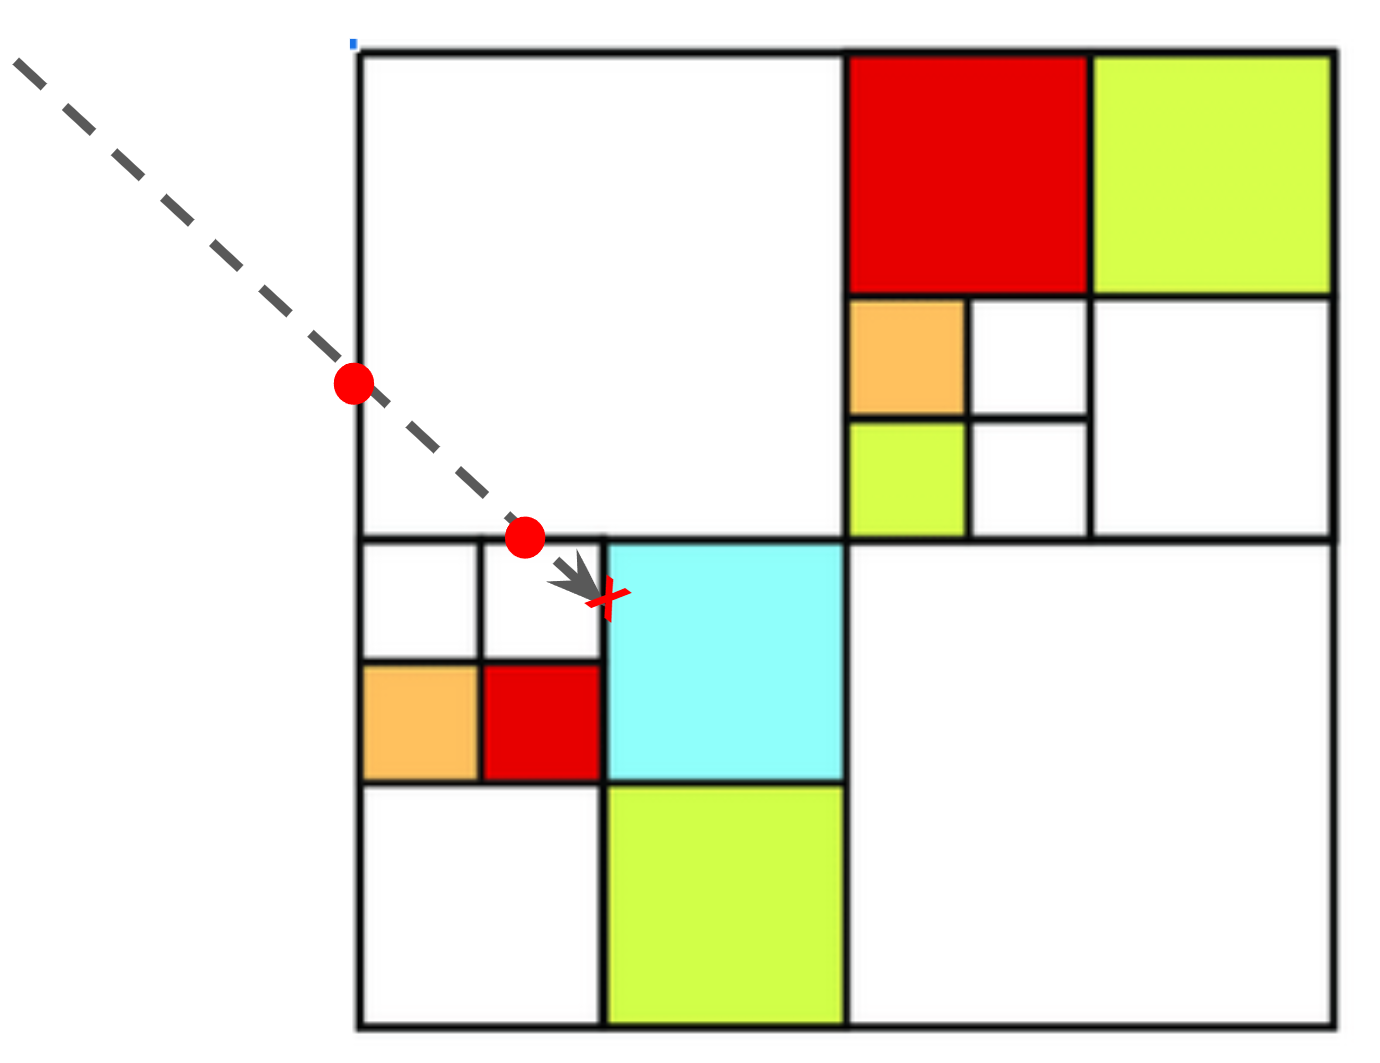
\includegraphics[width=.8\linewidth]{trace}
	\caption{Illustration of the path a ray will take when traversing a sparse voxel octree data structure. As a ray enters a larger voxel, it takes a longer step, resulting in fewer total traversals through the octree.}
	\label{fig:trace}
\end{figure}

\begin{figure}
	\centering
	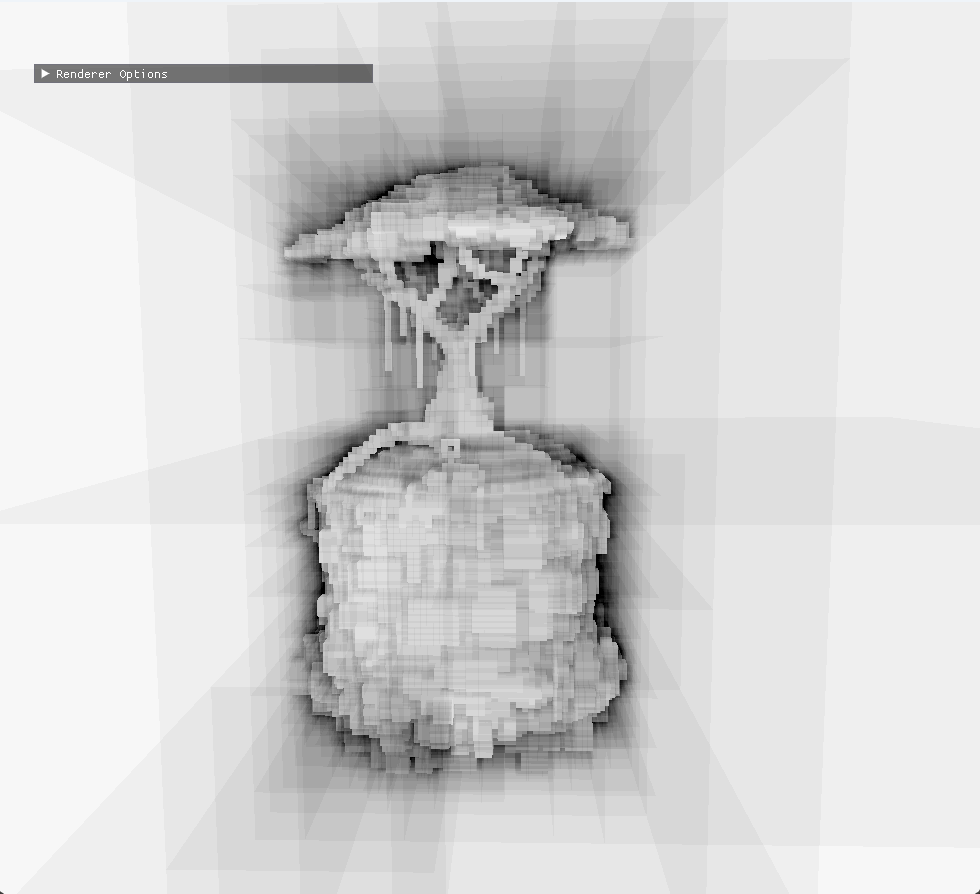
\includegraphics[width=1\linewidth]{depth}
	\caption{A visualization showing how more traversal steps are required near geometry, due to the sparsity of octree requiring smaller subdivisions.}
	\label{fig:depth}
\end{figure}
Throughout the algorithm I have used integers to approximate locations within the octree. As soon as the algorithm enters the octree which can be at any point in space, all points are transformed into the unit cube. From there three 32 bit values can represent any coordinate in the unit cube down to a precision of $2^{-32}$. The encoding for this format is such that the first bit represents $\frac12$, the next $\frac14$ and so on. This makes it easy to check what octant contains a certain point down to a specific depth, as the single bit representing an octree depth can just be checked. Furthermore, divisons by two can be heavily optimized as it just becomes a bit-shift operation, whereas with floating point a division is an awfully slow operation, even on GPU's which otherwise have very fast floating point arithmetic performance. The performance with and without coordinate-integer conversions was compared and the integer version performed roughly 20\% better at all resolution.








\subsection*{Scene Loading}
An initial test scene for development was created by sampling 3D-Perlin noise in a grid and placing voxels when the noise value passed a density threshold. The Perlin noise generator by \cite{perlin} was utilized. To load more structured scenes, an open source loader for Magicavoxel files from OpenGameTools \cite{OGT} was implemented, along with a translation layer. This enabled loading of entire Magicavoxel scenes with all the voxel colors and material appearance models - diffuse, metal, and glass - that matched those of Magicavoxel.

\subsection*{CPU Global Illumination}
To have something to compare to, and to test whether my octree traversal implementations and everything worked in an environment where everything could be debugged easily, I started out by implementing a CPU based voxel renderer. I got a bit carried away as, when I already had the intersect function, alculation of global illumination using Monte Carlo path tracing is quite easy and just requires more rays. I can then save the render to an accumulation buffer to minimize variance in the image over time. The different Bidirectional Reflectance Distribution Functions (BRDFs) which I have implemented thus far include diffuse, reflection and refraction shaders. A material index in the voxel data determines which sampling function to use for the succeeding ray. Diffuse rays are sampled from a cosine hemisphere and rotated to the normal \cite{ROTATE}. For reflected rays, the direction is mirrored along the normal, with fuzz added per material. Refracted rays have their direction calculated from the ratio of refractive indices. To trace inside voxels, the operation of the intersection algorithm is switched to its inverse, such that it returns when \textbf{not} hitting a voxel. This may also be used as an optimization for memory in very dense scenes. Upon hitting an emitter, the ray returns the attenuated luminance. As the cpu renderer runs at extremely low framerates, I chose to implement Intel's OpenImageDenoiser. With that implemeneted it only takes a couple of frames for the image to somewhat converge in the simpler scenes with mostly diffuse lighting.

\section{Results}
\subsection*{Performance}
The performance of the CPU ray tracer is understandably quite poor, but it was never meant to be anything more than a stepping stone. As I never got to implement either path tracing or cone tracing in my GPU implementation, it can only really be compared to the single hit cpu shader. In table \ref{tab:performance} below and the frametime graph in figure \ref{fig:times}, it can clearly be seen that even though all versions of the program scale linearly with the amount of pixels (rays cast per frame), the GPU version is able to do this much faster and more efficiently. The GPU renderer even becomes faster relative to the CPU implementation as the resolution increases, due to the waiting for the cpu taking up less time. At 720p it's 13 times faster while at 4k it's 21 times faster. The total power draw of my system as measured by HWInfo was also lower while running the GPU renderer. This is probably due to my GPU having a very limited TDP and therefore being current limited, while the CPU on all cores is able to boost higher. 
\begin{table}
	\begin{tabular}{lllll}
		\textbf{Resolution}               & 720p   & 1080p  & 1440p  & 2160p  \\ \hline
		\textbf{CPU {[}fps{]}}            & 55.00  & 26.00  & 12.90  & 6.60   \\
		\textbf{CPU GI {[}fps{]}}         & 11.50  & 5.00   & 2.80   & 1.50   \\
		\textbf{CPU GI Denoise {[}fps{]}} & 2.80   & 0.80   & 0.50   & 0.26   \\
		\textbf{GPU {[}fps{]}}            & 700.00 & 400.00 & 240.00 & 140.00
	\end{tabular}
	\caption{Comparison of framerates when running the different version of the program. CPU is a single hit shader, CPU GI uses Monte Carlo path tracing, CPU GI Denoise adds the ai denoiser to that and finally GPU is the single hit GPU tracer.}
	\label{tab:performance}
\end{table}
% TODO: \usepackage{graphicx} required
\begin{figure}
	\centering
	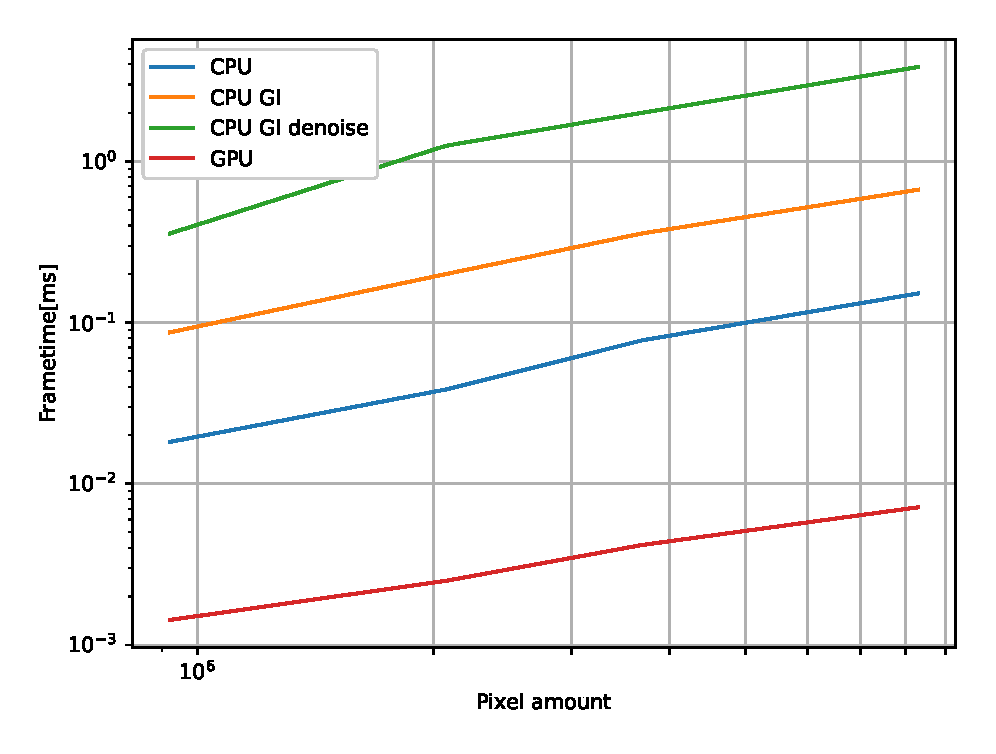
\includegraphics[width=0.8\linewidth]{times}
	\caption{Comparison of frametimes/pixel for the different rendering techniques. Both axes are in log scale.}
	\label{fig:times}
\end{figure}
\subsection*{Renders}
Sadly, the global illumination renderer looks much better than what I had time to do on the GPU. Even though the framerate was generally low, with the denoiser enabled it converged within a couple of seconds. If you don't care about real time performance or creating animations, the CPU based renderer might as well be the only thing you have. The only case where I see it being annoying is if you wanted to to modelling while showing the preview in real time, which is a luxury that some people have come to expect. Two cpu renders are shown in figures \ref{fig:cpu-close} and \ref{fig:cpu-far} and a gpu render with a single additional shadow ray is shown in figure \ref{fig:gpu-far}.
\begin{figure}
	\centering
	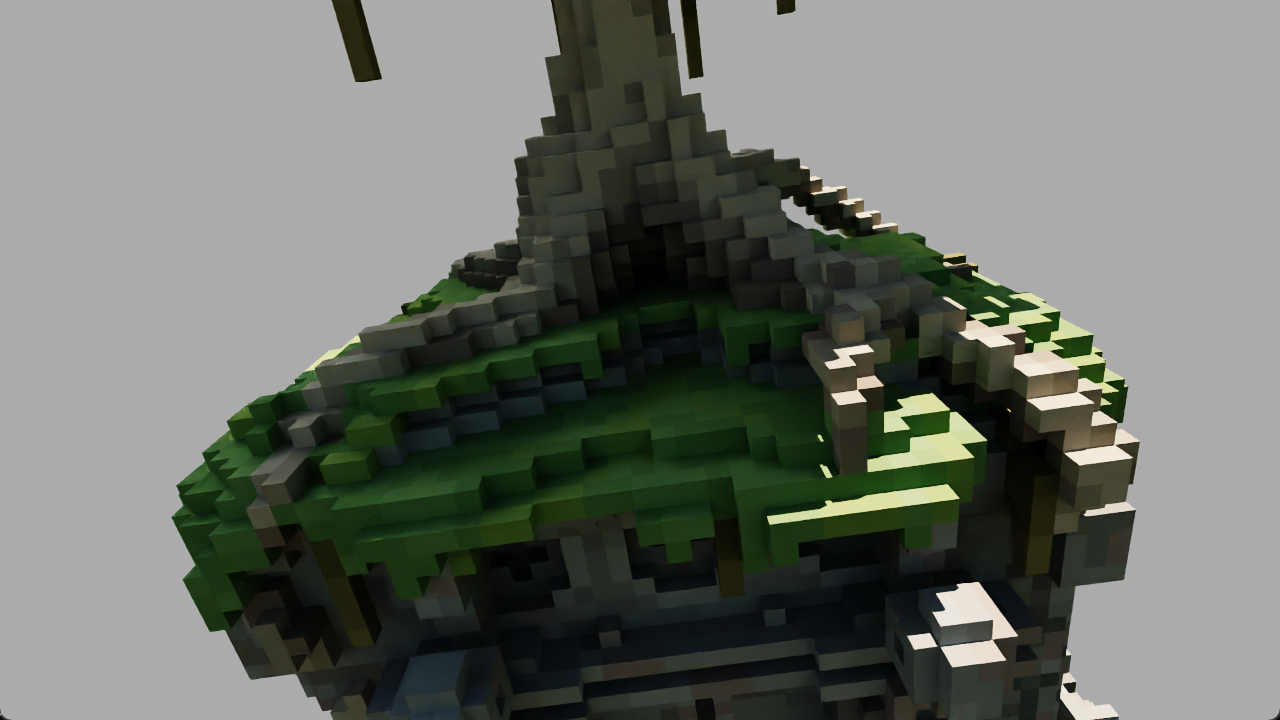
\includegraphics[width=1\linewidth]{Cpu-close}
	\caption{CPU-GI-Denoised render}
	\label{fig:cpu-close}
\end{figure}
% TODO: \usepackage{graphicx} required
\begin{figure}
	\centering
	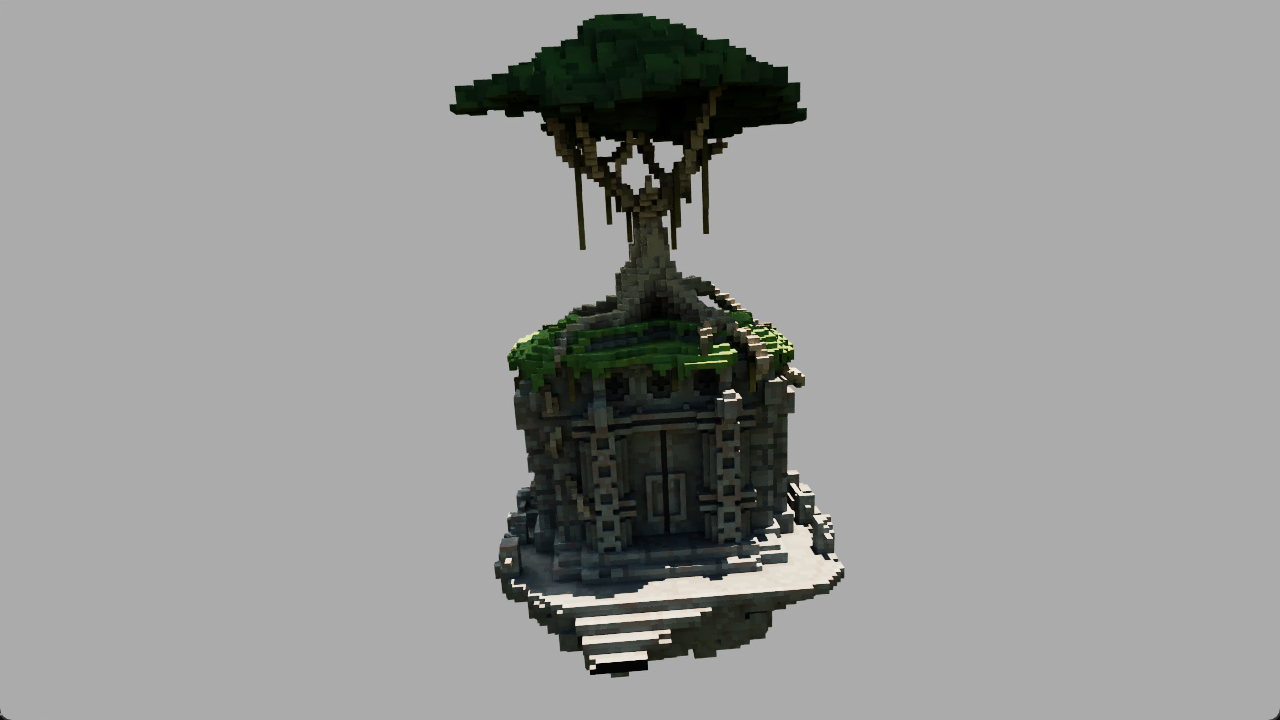
\includegraphics[width=1\linewidth]{cpu-far}
	\caption{CPU-GI-Denoised render}
	\label{fig:cpu-far}
\end{figure}

% TODO: \usepackage{graphicx} required
\begin{figure}
	\centering
	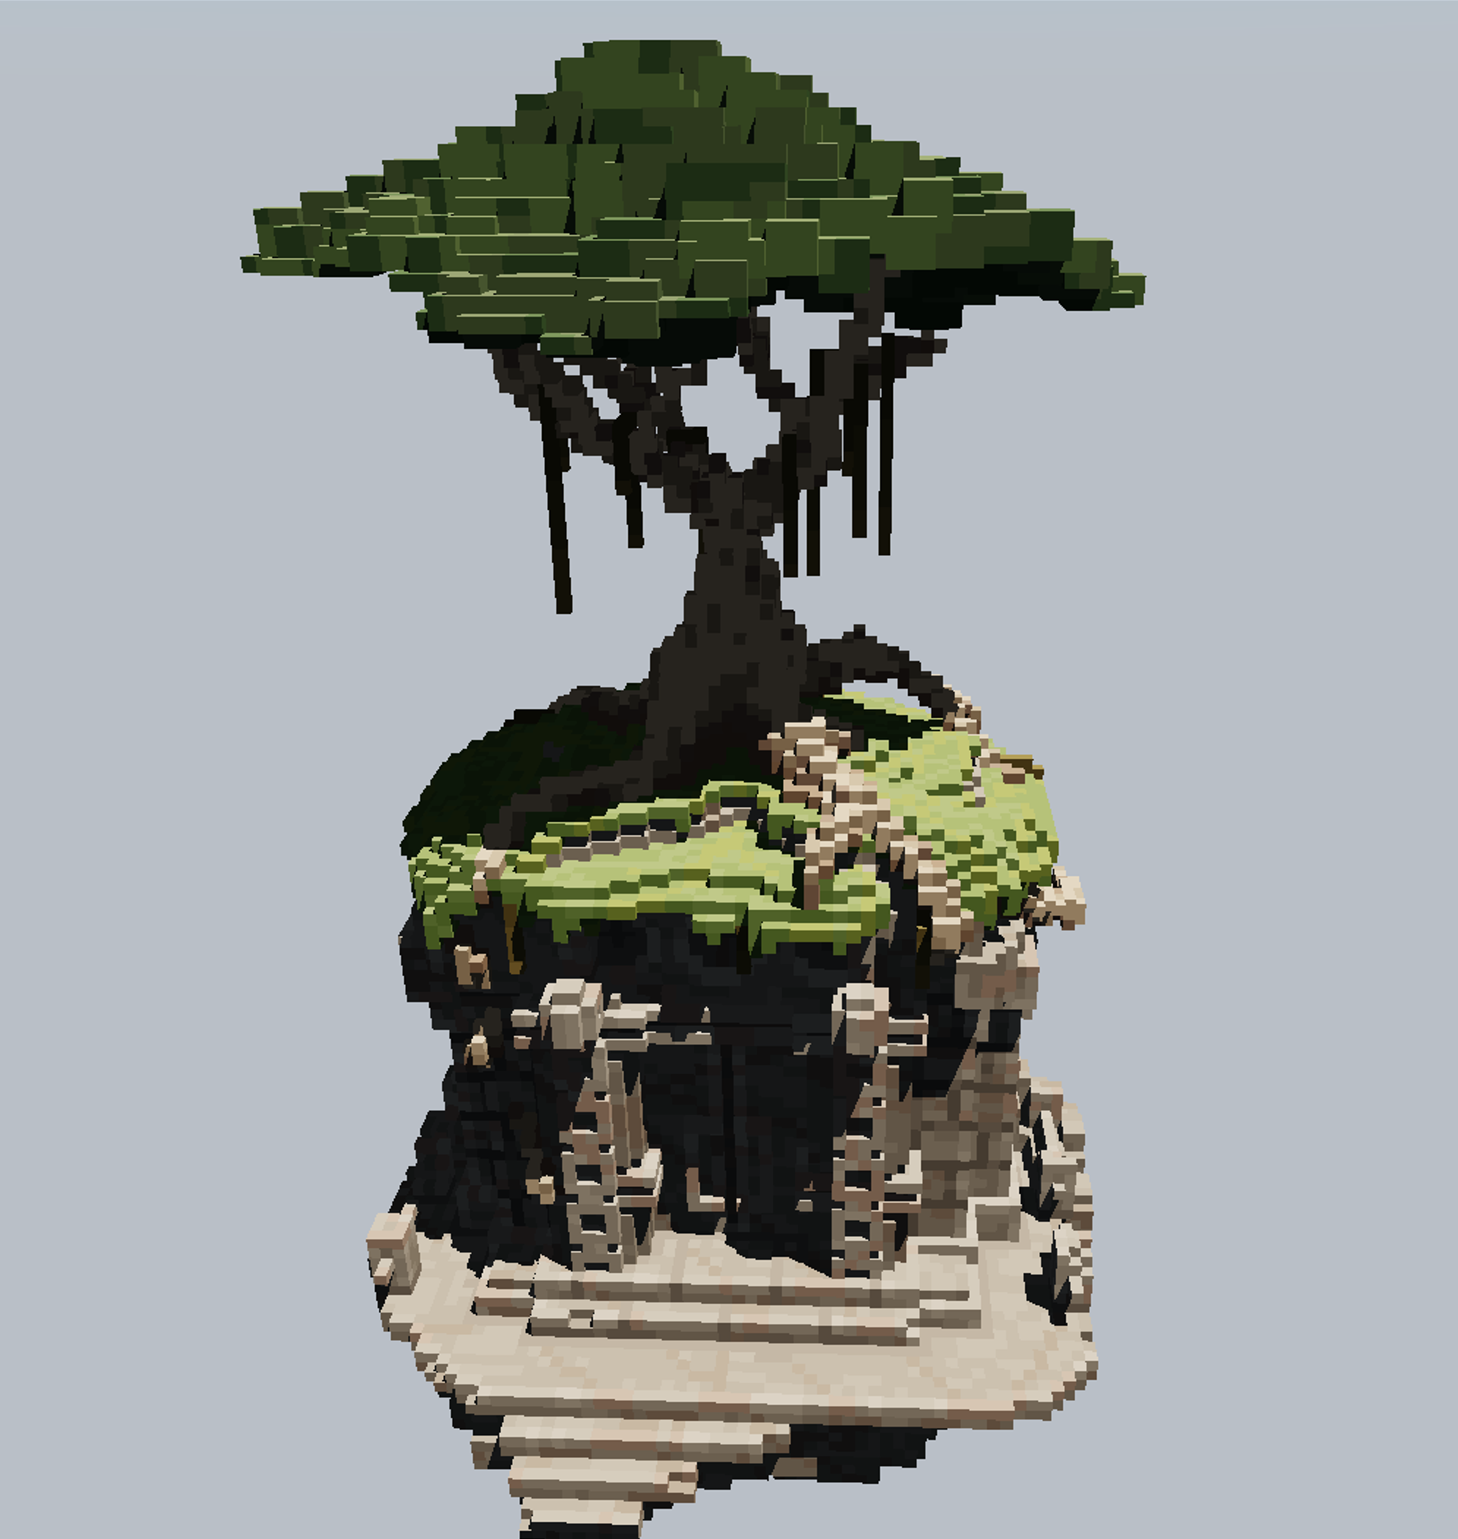
\includegraphics[width=1\linewidth]{gpu-far}
	\caption{GPU render}
	\label{fig:gpu-far}
\end{figure}


\section{Future Work}
The main area that I want to continue working on is of course to implement voxel cone tracing. I am planning on creating two shaders, one for accurate path-tracing and one with the approximated cone tracing, just so that I can compare the tradeoffs of the two. This does not seem to be a hard problem to tackle as the preliminary groundwork has been laid, I just need to put in the work. After that, I plan on implementing filtering techniques to reduce the variance of the output for better real-time performance. I have been looking into temporospatial filtering, which seems to be very useful in this instance. I also want to further utilize the fact that I am rendering voxels. There is hardware support for AABB intersections on the GPU ray tracing cores. Tracing into an octree is in essence a lot of AABB intersection checks, along with tree traversal, so perhaps that can be utilized. I would also like to try adding neighbour node pointers to my octree. These would of course have to be signed offsets as sometime you have to go back in the gridpool to find a neighbour. So all in all there is a lot of stuff left to do, and I will continue working on this codebase as I find it very fun.
% Bibliography
\bibliographystyle{ACM-Reference-Format}
\bibliography{voxeltrace_paper_bibliography}

	
	
	
\end{document}
